\documentclass[journal,12pt,two column]{IEEEtran}


\usepackage{listings}
\usepackage{amssymb}
\usepackage[cmex10]{amsmath}
\usepackage{amsthm}
\usepackage[export]{adjustbox}
\usepackage{bm}
\def\inputGnumericTable{} 

\usepackage[latin1]{inputenc}                                 
\usepackage{color}                                            
\usepackage{array}   
\usepackage{longtable}
\usepackage{enumitem}
\usepackage{calc}                                             
\usepackage{multirow}                                         
\usepackage{hhline}                                           
\usepackage{ifthen}  
\usepackage{mathtools}
\usepackage{tikz}
\usepackage{listings}
\usepackage{color}                                            %%
\usepackage{array}                                            %%
\usepackage{caption} 
\usepackage{graphicx}
\graphicspath{{images/}}
\newcommand*{\permcomb}[4][0mu]{{{}^{#3}\mkern#1#2_{#4}}}
\newcommand*{\perm}[1][-3mu]{\permcomb[#1]{P}}\usepackage{setspace}
%\captionsetup[table]{skip=3pt} 

\title{AI1110 Assignment  }
\author{Tejal Kulkarni \\ CS21BTECH11058 \\\vspace*{20pt} June 2022 \\  Probability Assignment}

\begin{document}
\maketitle

\newcommand{\solution}{\noindent \textbf{Solution: }}
\providecommand{\pr}[1]{\ensuremath{\Pr\left(#1\right)}}
\providecommand{\cdf}[2]{\ensuremath{\text{F}_{#1}\left(#2\right)}}
\providecommand{\qfunc}[1]{\ensuremath{Q\left(#1\right)}}
\providecommand{\sbrak}[1]{\ensuremath{{}\left[#1\right]}}
\providecommand{\lsbrak}[1]{\ensuremath{{}\left[#1\right.}}
\providecommand{\rsbrak}[1]{\ensuremath{{}\left.#1\right]}}
\providecommand{\brak}[1]{\ensuremath{\left(#1\right)}}
\providecommand{\lbrak}[1]{\ensuremath{\left(#1\right.}}
\providecommand{\rbrak}[1]{\ensuremath{\left.#1\right)}}
\providecommand{\cbrak}[1]{\ensuremath{\left\{#1\right\}}}
\providecommand{\lcbrak}[1]{\ensuremath{\left\{#1\right.}}
\newcommand*{\comb}[1][-1mu]{\permcomb[#1]{C}}
\renewcommand{\thetable}{\arabic{table}}
\providecommand{\rcbrak}[1]{\ensuremath{\left.#1\right\}}}
\newcommand{\myvec}[1]{\ensuremath{\begin{pmatrix}#1\end{pmatrix}}}
\newcommand{\mydet}[1]{\ensuremath{\begin{vmatrix}#1\end{vmatrix}}}
\let\vec\mathbf

\textbf{1.3:} Find a theoretical expression for $F_U(x)$

\solution

\begin{align}  
f_{U}\brak{x} = 
\begin{cases}
1, & x\in (0,1) \\
0, & \text{otherwise}
\end{cases}
\end{align}
\begin{equation}
    F_U(x) = \int_{-\infty}^{x} f_{U}\brak{x} \,dx  \\
\end{equation}
Hence,
If $ x \leq 0 $,
\begin{align}
    F_U(x) &= \int_{-\infty}^{x} f_{U}\brak{x} \,dx  \\
    F_U(x) &= \int_{-\infty}^{x} 0 \,dx  \\
           &= 0
\end{align}
If $0 <x <1$,
\begin{align}
    F_U(x) &= \int_{0}^{x} f_{U}\brak{x} \,dx  \\
    F_U(x) &= \int_{0}^{x} 1 \,dx  \\
           &= x
\end{align}
If $x \geq 1$,
\begin{align}
    F_U(x) &= \int_{1}^{x} f_{U}\brak{x} \,dx  \\
    F_U(x) &= \int_{1}^{x} 0 \,dx  \\
           &= 0
\end{align}
Hence,
\begin{align}  
F_{U}\brak{x} = 
\begin{cases}
x, & x\in (0,1) \\
0, & \text{otherwise}
\end{cases}
\end{align}
\begin{figure}[!ht]
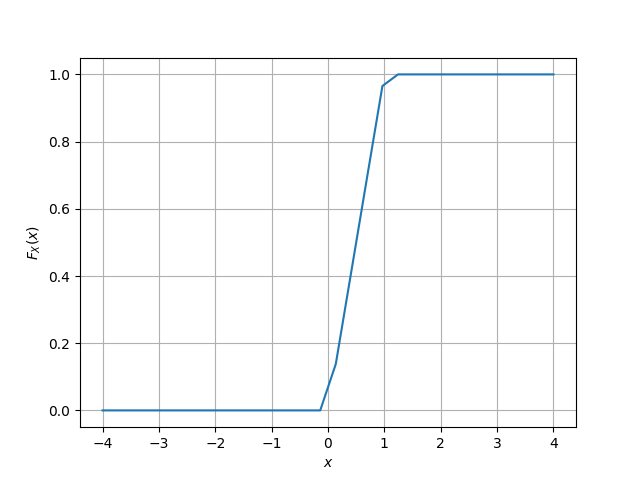
\includegraphics[width = \columnwidth]{U_CDF.png}
\caption{CDF of U}
\label{Fig 1}
\end{figure}   

\textbf{1.5:} Verify your result theoretically given that,
\begin{equation}
    E\sbrak{U^k} = \int_{-\infty}^{\infty} x^k \,dF_{U}\brak{x}
\end{equation}

\solution

\begin{align}
    E\sbrak{U^k} &=  0 + \int_{0}^{1} x^k \,dF_{U}\brak{x} + 0 \\
                 &= \frac{1}{k + 1}  \\
    \implies E\sbrak{U} &= \frac{1}{2}\\
                        &= 0.50 \\
             E\sbrak{U^2} &= \frac{1}{3}
\end{align}
Hence,
\begin{align}
    \text{variance} &= E\sbrak{U^2} - \brak{E\sbrak{U}}^2 \\
                    &= \frac{1}{3} - \brak{\frac{1}{2}}^2 \\
                    &= \frac{1}{12} \\
                    &= 0.0833
\end{align}

\textbf{2.2:} What properties does a CDF have?

\solution
The CDF of a random variable U has the following properties:
\begin{enumerate}
    \item $F_{U}\brak{x}$ is a non decreasing function of x where $-\infty < x < \infty$ 
    \item $F_{U}\brak{x}$ ranges from 0 to 1 
    \item $F_{U}\brak{x} = 0$ as $x \rightarrow -\infty$ 
    \item $F_{U}\brak{x} = 1$ as $x \rightarrow \infty$
\end{enumerate}

\textbf{2.3:} What properties does a PDF have?

\solution
The PDF of a random variable X has the following properties:
\begin{enumerate}
    \item The probability density function is non-negative for all the possible values. \\
    \item $ \int_{-\infty}^{\infty} f\brak{x} \,dx  = 1 $ 
    \item $f\brak{x} = 0$ as $x \rightarrow -\infty$
    \item $f\brak{x} = 0$ as $x \rightarrow \infty$
\end{enumerate}

\textbf{2.5:} Given that
\begin{equation}
    p_{X}\brak{x} = \frac{1}{\sqrt{2\pi}}exp\brak{-\frac{x^2}{2}} ,  -\infty < x < \infty
\end{equation}
repeat the above exercise theoretically.

\solution
By definition,
\begin{equation}
    p_{X}\brak{x}dx = dF_{U}\brak{x}
\end{equation}
Hence,
\begin{align}
    E\sbrak{U} &= \int_{-\infty}^{\infty} x p_{X}\brak{x} \,dx \\
               &= \int_{-\infty}^{\infty} x \frac{1}{\sqrt{2\pi}}exp\brak{-\frac{x^2}{2}} \,dx \\
               &= 0
\end{align}
Also,
\begin{equation}
    \text{variance} = E\sbrak{U^2} - \brak{E\sbrak{U}}^2
\end{equation}
\begin{align}
   E\sbrak{U^2} &=  \int_{-\infty}^{\infty} x^2 p_{X}\brak{x} \,dx \\
                &= \int_{-\infty}^{\infty} x^2 \frac{1}{\sqrt{2\pi}}exp\brak{-\frac{x^2}{2}} \,dx \\
                &= 1 \\
    \implies \text{variance} = 1
\end{align}
Also,
\begin{align}
   F_{U}\brak{x} &=  \int_{-\infty}^{x} p_{X}\brak{x} \,dx  \\
                 &= \int_{-\infty}^{x} e^{-\frac{x^2}{2}}\,dx 
\end{align}
\begin{figure}[!ht]
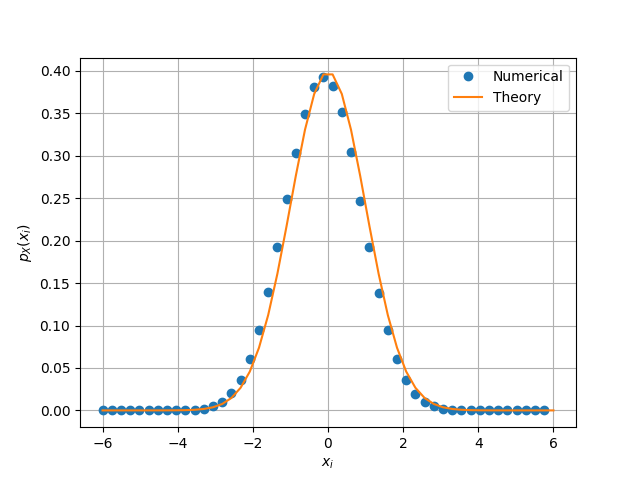
\includegraphics[width = \columnwidth]{X_PDF.png}
\caption{PDF of X}
\label{Fig 2}
\end{figure}  
\begin{figure}[!ht]
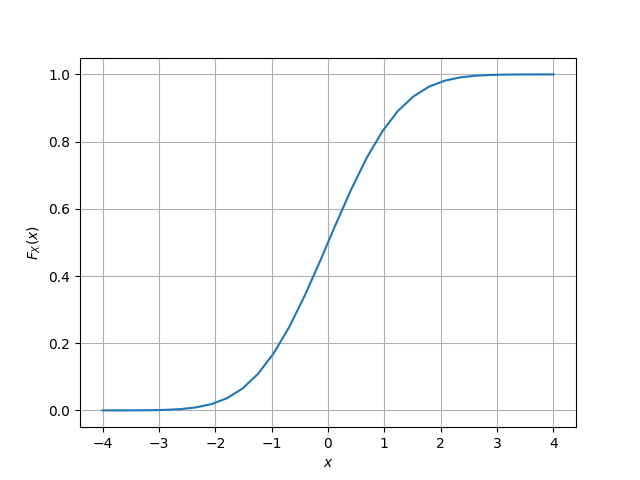
\includegraphics[width = \columnwidth]{X_CDF.png}
\caption{CDF of X}
\label{Fig 3}
\end{figure}  


\textbf{3.2:} Find a theoretical expression for $F_V\brak{x}$

\solution
Let, $V = g\brak{U}$
\begin{align}
    V &= -2\ln{(1 - U)} \\
    \implies U &= 1 - e^{-\frac{V}{2}}
\end{align}
Now, 
\begin{align}
    F_{V}\brak{x} &= P\brak{g\brak{U}\leq x} \\
                  &= P\brak{X < g^{-1}\brak{V}} \\
                  &= F_{U}\brak{g^{-1}\brak{V}} \\
                  &= F_{U}\brak{1 - e^{-\frac{V}{2}}}
\end{align}
\begin{align}  
F_{U}\brak{1 - e^{-\frac{V}{2}}} = 
\begin{cases}
1 - e^{-\frac{V}{2}}, & V \in (0,\infty) \\
0, & \text{otherwise}
\end{cases}
\end{align}
\begin{figure}[!ht]
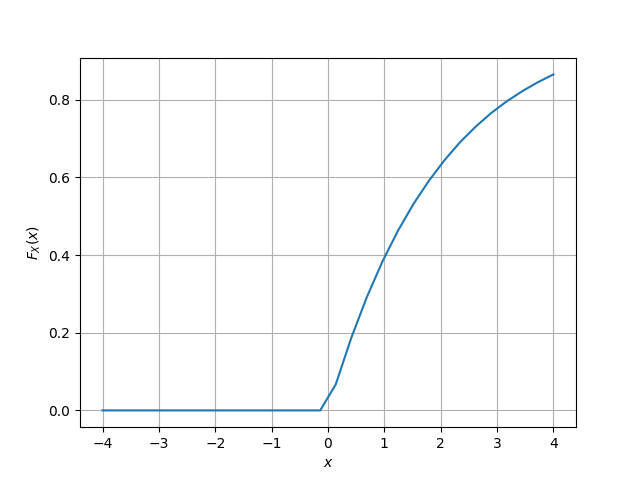
\includegraphics[width = \columnwidth]{V_CDF.png}
\caption{CDF of V}
\label{Fig 4}
\end{figure}   


\end{document}
